\documentclass[border=15pt, multi, tikz]{standalone}
\usepackage{import}
\usepackage{etoolbox}
\usepackage{graphicx}
\usepackage{svg}
\usepackage{colortbl}

\usetikzlibrary{positioning,matrix,fit}
\usetikzlibrary{3d} %for including external image
\usetikzlibrary{decorations,shapes}
\usetikzlibrary{decorations.shapes}
\usetikzlibrary{decorations.markings}
\usetikzlibrary{decorations.pathreplacing}
\usetikzlibrary{backgrounds}
\usetikzlibrary{calc}
\usetikzlibrary{arrows.meta,arrows}
\graphicspath{{image/}}

\tikzset{%
  % Specifications for style of nodes:
    >={Latex[width=2mm,length=2mm]},
}

\begin{document}
  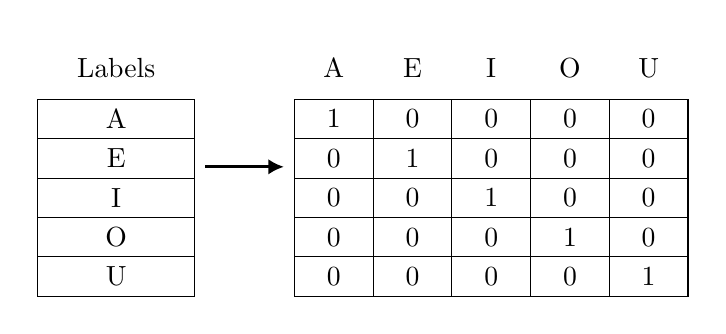
\begin{tikzpicture}
    \matrix (v) [matrix of nodes, row sep=-\pgflinewidth, column sep=-\pgflinewidth,
        nodes={minimum height = 5mm, minimum width = 2cm, outer sep=0, anchor=center, draw},
        nodes in empty cells,
        row 1/.style={nodes={draw=none,minimum height=8mm}},
        e/.style={fill=yellow!10}
      ]
      {
        Labels\\
        A\\
        E\\
        I\\
        O\\
        U\\
      };
      \matrix (hot) [right=of v, matrix of nodes, row sep=-\pgflinewidth, column sep=-\pgflinewidth,
        nodes={minimum height = 5mm, minimum width = 1cm, outer sep=0, inner sep=0, anchor=center, draw},
        row 1/.style={nodes={draw=none,minimum height=8mm}},
        nodes in empty cells,
        e/.style={fill=yellow!10}
      ]
      {
        A & E & I & O & U\\
        1 & 0 & 0 & 0 & 0\\
        0 & 1 & 0 & 0 & 0\\
        0 & 0 & 1 & 0 & 0\\
        0 & 0 & 0 & 1 & 0\\
        0 & 0 & 0 & 0 & 1\\
      };
      \draw[->,very thick] (v) -- (hot);
  \end{tikzpicture}
\end{document}